\documentclass[11pt]{article}
\usepackage{amssymb}
\usepackage{tikz}
\usepackage{fancyhdr}
\usepackage{extramarks}
\usepackage{pgfplots}
\usetikzlibrary{automata,positioning}
\usetikzlibrary{shapes.geometric, arrows}


\setlength{\topmargin}{-1.5in}
\setlength{\textheight}{9.5in}
\setlength{\oddsidemargin}{.125in}
\setlength{\textwidth}{6.25in}

\tikzstyle{startstop} = [rectangle, rounded corners, minimum width=3cm, minimum height=1cm,text centered, text width=3cm, draw=black, fill=red!30]
\tikzstyle{planned} = [rectangle, minimum width=3cm, minimum height=1cm,text centered, text width=3cm, draw=black, fill=green!30]
\tikzstyle{current} = [rectangle, minimum width=3cm, minimum height=1cm,text centered, text width=3cm, draw=black, fill=red!30]

\tikzstyle{io} = [trapezium, trapezium left angle=70, trapezium right angle=110, minimum width=3cm, minimum height=1cm, text centered, text width=2cm,draw=black, fill=blue!30]
\tikzstyle{process} = [rectangle, minimum width=3cm, minimum height=1cm, text centered, text width=2cm,draw=black, fill=orange!30]
\tikzstyle{decision} = [diamond, minimum width=3cm, minimum height=1cm, text centered, text width=2cm, draw=black, fill=green!30]



\tikzstyle{arrow} = [thick,->,>=stealth]
\begin{document}
	\title{
		\textbf{Car Logic Implementation}
	}
	\date{}
	\maketitle

\begin{center}
	\begin{tikzpicture}[node distance=2.5cm]



	\node (carLogicAPI)[planned, xshift=3cm]{Car Logic API};

	\node (autoDriver) [current, below of=carLogicAPI, xshift=-3cm] {Auto Driver};
	\node (hardware)[current, below of=autoDriver] {Sensors / Inputs};

	\node(meshAPI)[planned, below of=carLogicAPI, xshift=3cm]{Mesh Network};
	\node(netHardware)[planned, below of=meshAPI] {Networking Hardware};



	\draw [arrow] (hardware.110) -- (autoDriver.250);
	\draw [arrow] (autoDriver.290) -- (hardware.70);

	\draw [arrow] (autoDriver.110) |- (carLogicAPI.170);
	\draw [arrow] (carLogicAPI.190) -| (autoDriver.70);

	\draw [arrow] (netHardware.110) -- (meshAPI.250);
	\draw [arrow] (meshAPI.290) -- (netHardware.70);

	\draw [arrow] (carLogicAPI.10) -| (meshAPI.70);
	\draw [arrow] (meshAPI.110) |- (carLogicAPI.350);

	\end{tikzpicture}
\end{center}

	\begin{enumerate}
		\item Hardware sensors: These are various data collection tools installed
			on the car, like compass, cameras, lidar and sonar, accelerometers,
			and any other sensors. The inputs are things like the braking,
			acceleration, steering, and lights.
		\item Autonomous driver: This manufacturer specific implementation
			is the interpretation of the raw input into abstract descriptions,
			such as lane position, position of other cars, and current direction
			and route. Also in this block would be the code to control the car,
			such as how to maintain a lane, how to set a speed, how to shift a lane.
			Also it should have safety checks, like preventing collisions, avoiding
			objects, and limiting turning speed. These parts are already in
			self-driving cars. They will also need to add the calls to the Car Logic API,
			and decide what to do with that data and whether to follow the suggestions.
		\item Car Logic API: The goal of this project. The idea here is to create a
			shared library that all manufacturers can implement parts of, and
			so that the cars on the road can collaborate, whether
			or not they are the same model, manufacturer, or even whether or not they
			are self-driving cars. The goal here is to make it standard, and modular, so that
			the choice of how to implement and how much to implement, is left up to
			the manufacturer, that way they can make luxury models, budget models,
			improve, expand, and all while still being able to communicate with other
			cars on the road.
		\item Mesh Network: This software allows the cars to form a mesh network, so that
			messages from any car can get to any other car in the mesh network. Most
			of the uses will be to transmit to cars immediately around the source, so
			long communication routes would be rare.
		\item Network hardware: This equipment allows for the transmission and
			reception of packets on some radio signal range. Targets include other
			cars, but also intelligent installations such as "caches" of accumulated
			data, traffic signals, repeaters, or smart road sections. Cars could use
			IEEE 802.11p / IEEE 1609 WAVE or other forms of wireless communication.
	\end{enumerate}
\end{document}
